\section{Experimental Modeling}
\label{ch:experimental-modeling}

This section describes the protocol model, static checker rules, and evaluation plan for hypotheses H1--H4 (Section~\ref{ch:related-work}). All checks target synchronous C++ gRPC streaming endpoints (\texttt{ClientReader}, \texttt{ClientWriter}, \texttt{ClientReaderWriter}, \texttt{ServerReader}, \texttt{ServerWriter}, and \texttt{ServerReaderWriter}), leaving aside asynchronous \texttt{CompletionQueue} tags and callback reactors.

\subsection{System Architecture and Structured AST Pipeline}
\label{sec:exp-architecture}

Checking runs in three stages (Figure~\ref{fig:dataflow}). We read the Clang C++ AST instead of LLVM IR, GCC GIMPLE, or \texttt{clang::CFG} because source AST nodes still expose C++ templates and Protobuf setter calls before optimization lowers them away, while letting us time parsing and checking separately:
\begin{enumerate}
    \item \textbf{Schema and Standard Codegen:} Service \texttt{.proto} files define RPCs, \texttt{oneof} choices, and optional \texttt{MethodOptions} contracts beside each RPC without modifying \texttt{protoc}; standard \texttt{protoc} produces the normal C++ headers.
    \item \textbf{Contract Compiler:} A standalone compiler parses each \texttt{MethodOptions} string, flips it via duality ($\overline{S}$) for the server, verifies determinism, and writes \texttt{grpc.session.v1} JSON automata containing \texttt{protocol} metadata (\texttt{method\_aliases}, \texttt{handler\_sequence}), \texttt{initial\_state}/\texttt{terminal\_states}, transitions (\texttt{states}), \texttt{payload\_setters}, and \texttt{payload\_groups} (\texttt{"type":"all"} combined guards).
    \item \textbf{Clang AST Checker:} \texttt{clang++} parses each unmodified C++17 file (\texttt{-Xclang -ast-dump=json -fsyntax-only}), and a standalone checker walks the AST directly to track branches, loops, \texttt{break}/\texttt{continue}, returns, \texttt{try}/\texttt{catch}, and \texttt{throw}. Whenever an RPC has no custom option, the checker uses a universal Level~1 stream automaton.
\end{enumerate}

\begin{figure}[htbp]
\centering
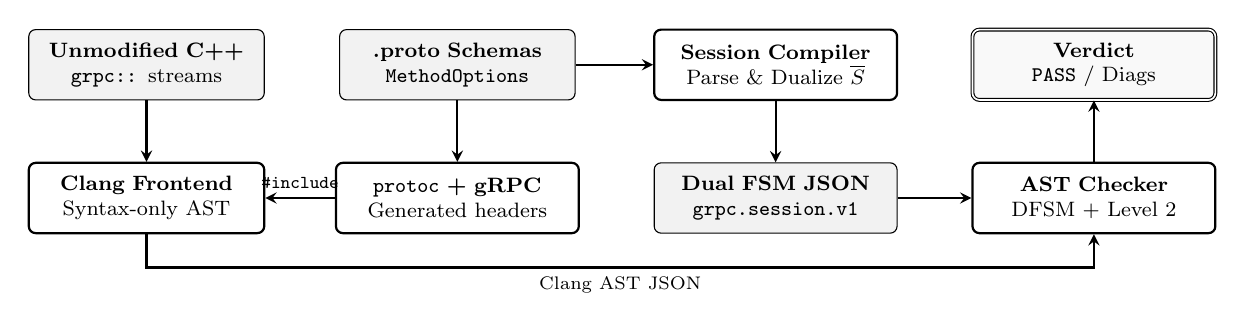
\begin{tikzpicture}[
    scale=0.94, transform shape,
    >=stealth,
    nodebox/.style={draw, rounded corners=2.5pt, align=center, font=\footnotesize, minimum height=0.95cm, inner sep=4pt},
    data/.style={nodebox, fill=gray!10},
    proc/.style={nodebox, fill=white, thick},
    outbox/.style={nodebox, double, fill=gray!5}
]
    \node[data, text width=2.9cm] (cpp)    at (0.0,  1.8) {\textbf{Unmodified C++}\\\texttt{grpc::} streams};
    \node[data, text width=2.9cm] (proto)  at (4.2,  1.8) {\textbf{.proto Schemas}\\\texttt{MethodOptions}};
    \node[proc, text width=3.0cm] (protoc) at (4.2,  0.0) {\textbf{\texttt{protoc} + gRPC}\\Generated headers};
    \node[proc, text width=3.0cm] (comp)   at (8.5,  1.8) {\textbf{Session Compiler}\\Parse \& Dualize $\overline{S}$};
    \node[data, text width=3.0cm] (fsm)    at (8.5,  0.0) {\textbf{Dual FSM JSON}\\\texttt{grpc.session.v1}};
    \node[proc, text width=2.9cm] (clang)  at (0.0,  0.0) {\textbf{Clang Frontend}\\Syntax-only AST};
    \node[proc, text width=3.0cm] (verif)  at (12.8, 0.0) {\textbf{AST Checker}\\DFSM + Level~2};
    \node[outbox, text width=3.0cm] (diag) at (12.8, 1.8) {\textbf{Verdict}\\\texttt{PASS} / Diags};

    \draw[->, thick] (proto.south)  -- (protoc.north);
    \draw[->, thick] (proto.east)   -- (comp.west);
    \draw[->, thick] (comp.south)   -- (fsm.north);
    \draw[->, thick] (cpp.south)    -- (clang.north);
    \draw[->, thick] (protoc.west)  -- node[above, font=\scriptsize] {\texttt{\#include}} (clang.east);
    \draw[->, thick] (clang.south)  -- +(0,-0.45) -| node[pos=0.25, below, font=\scriptsize] {Clang AST JSON} (verif.south);
    \draw[->, thick] (fsm.east)     -- (verif.west);
    \draw[->, thick] (verif.north)  -- (diag.south);
\end{tikzpicture}
\caption{Verification pipeline linking standard \texttt{protoc} codegen, dual DFSM synthesis, and structured Clang AST checking.}
\label{fig:dataflow}
\end{figure}

\subsection{Formal Behavioral Model and Lifecycle Semantics}
\label{sec:exp-formalism}

\paragraph{Endpoint Grammars, Operations, and Duality.}
Allowed C++ calls depend on stream direction: clients use \texttt{Read}, \texttt{Finish}, and \texttt{TryCancel} (server-streaming); \texttt{Write}, \texttt{WritesDone}/\allowbreak\texttt{WriteLast}, \texttt{Finish}, and \texttt{TryCancel} (client-streaming); or all five (bidirectional). Servers use \texttt{Write} (server-streaming), \texttt{Read} (client-streaming), or both (bidirectional) before returning a \texttt{grpc::\allowbreak Status} (servers have no \texttt{WritesDone()}). We distinguish the author-written \textbf{client grammar} $S_{\mathrm{client}}$ from the compiler-derived \textbf{server grammar} $S_{\mathrm{server}} = \overline{S_{\mathrm{client}}}$:
\begin{equation}
\label{eq:session-grammar}
\begin{aligned}
S_{\mathrm{client}} &::=\; {!}T[\gamma]; S \;\mid\; {?}T[\gamma]; S \;\mid\; \oplus\{l_i : S_i\}_{i \in I} \;\mid\; \&\{l_i : S_i\}_{i \in I} \\
                   &\quad\;\mid\; \mu X. S \;\mid\; X \;\mid\; \mathsf{WritesDone}; S \;\mid\; \mathsf{ClientObserveStatus}(\varsigma) \;\mid\; \mathsf{end}, \\
S_{\mathrm{server}} &::=\; {?}T[\gamma]; S' \;\mid\; {!}T[\gamma]; S' \;\mid\; \&\{l_i : S'_i\}_{i \in I} \;\mid\; \oplus\{l_i : S'_i\}_{i \in I} \\
                   &\quad\;\mid\; \mu X. S' \;\mid\; X \;\mid\; \mathsf{PeerEndOfInput}; S' \;\mid\; \mathsf{ServerReturnStatus}(\varsigma) \;\mid\; \mathsf{end},
\end{aligned}
\end{equation}
where $T \in \mathcal{T}$ is a message type, $\gamma \in \Gamma \cup \{\bot\}$ is an optional Level~2 payload condition, $l_i \in \mathcal{L}$ are branch labels, $X \in \mathcal{X}$ are recursion variables, and $\varsigma \in \{\mathsf{OK}, \mathsf{ERR}\}$. When lowering $\mathsf{end}$, client paths finish with \texttt{Finish()} (reading \texttt{Read(eos)} first on \texttt{Read}/$\mathsf{end}$ branches), and server paths return \texttt{grpc::Status}. Endpoint duality $\overline{S}$ flips send/receive, selection/branching, half-close, and status handling:
\begin{align}
\overline{{!}T[\gamma]; S} &= {?}T[\gamma]; \overline{S}, &
\overline{{?}T[\gamma]; S} &= {!}T[\gamma]; \overline{S}, \nonumber \\
\overline{\oplus\{l_i : S_i\}} &= \&\{l_i : \overline{S_i}\}, &
\overline{\&\{l_i : S_i\}} &= \oplus\{l_i : \overline{S_i}\}, \nonumber \\
\overline{\mathsf{WritesDone}; S} &= \mathsf{PeerEndOfInput}; \overline{S}, &
\overline{\mathsf{ClientObserveStatus}(\varsigma)} &= \mathsf{ServerReturnStatus}(\varsigma), \label{eq:duality} \\
\overline{\mu X. S} &= \mu X. \overline{S}, &
\overline{X} = X, \qquad \overline{\mathsf{end}} &= \mathsf{end}. \nonumber
\end{align}
Multiple threads sharing one stream handle fall outside our sequential single-function scope (Section~\ref{sec:exp-boundaries}).

\paragraph{Stream Closure, Cancellation, and Error Outcomes.}
Our checker reacts to a tagged set of events (with $\omega \in \{\mathsf{ok}, \mathsf{fail}\}$, $\rho \in \{\mathsf{ok}, \mathsf{eos}, \mathsf{fail}\}$, and $\varsigma \in \{\mathsf{OK}, \mathsf{ERR}\}$):
\begin{equation}
\label{eq:alphabet}
\begin{aligned}
\Sigma = \bigl\{\,&
\mathsf{Write}(T, \gamma, \omega),\; \mathsf{Read}(T, \rho),\; \mathsf{HalfClose}(\omega),\; \mathsf{Finish}(\varsigma), \\
&\mathsf{CancelRequest},\; \mathsf{ServerReturn}(\varsigma),\; \mathsf{ServerCancelled}(\mathsf{bool})
\,\bigr\}.
\end{aligned}
\end{equation}
Matching \texttt{libgrpc++ 1.72.0}, closure and abort paths follow two rules:
\begin{itemize}
    \item \textbf{Client vs.\ Server \texttt{Read() == false}:} On a client, \texttt{Read(eos)} marks incoming data complete ($r_{\mathrm{in}}(v) = \mathsf{Yes}$) and still requires \texttt{Finish()}, whose status mixes server application errors with cancellation and network drops. On a server, \texttt{Read()} calls \texttt{MaybeMarkCancelledOnRead()} on \texttt{false}, so $\mathcal{M}_{\mathrm{srv}}(v)$ tracks why input stopped: $\mathsf{confirmed\_cancel}$ (\texttt{IsCancelled()} true, $F_{\mathrm{abort}}$), $\mathsf{confirmed\_norm}$ (\texttt{!IsCancelled()}), or $\mathsf{ambiguous}$ (idiomatic loops that omit \texttt{IsCancelled()}, allowed without false errors). Because $\mathcal{M}_{\mathrm{srv}}(v)$ is set only after \texttt{Read(eos)}, checking \texttt{!IsCancelled()} beforehand never claims $\mathsf{confirmed\_norm}$.
    \item \textbf{Write Failure, \texttt{WriteLast}, and Cancellation:} Only valid writes or half-closes that return \texttt{false} ($\omega = \mathsf{fail}$) count as $F_{\mathrm{abort}}$; illegal calls after close still report errors and cannot excuse missing cleanup. Client \texttt{WriteLast(m, opts)} and \texttt{set\_\allowbreak last\_\allowbreak message()} execute \texttt{Write(m); WritesDone()}; on servers, \texttt{WriteLast} records $v \in \mathcal{W}_{\mathrm{last}}$ and rejects any later writes before return. \texttt{ClientContext::\allowbreak TryCancel()} is best-effort ($v \in \mathcal{C}_{\mathrm{req}}$, allowing cleanup \texttt{Finish()}, not $F_{\mathrm{abort}}$), while \texttt{ServerContext::\allowbreak TryCancel()} (discouraged in \texttt{server\_\allowbreak context.h:213--214}) triggers an advisory warning and never satisfies normal return completion.
\end{itemize}

Compiled DFSMs separate termination outcomes by endpoint role:
\begin{equation}
\label{eq:dfsm-tuple}
M_r = (Q, \Sigma, \delta, q_0, F_{\mathrm{norm}}, F_{\mathrm{status\_nonOK}}, F_{\mathrm{app\_err}}, F_{\mathrm{abort}}), \qquad r \in \{\mathrm{client}, \mathrm{server}\},
\end{equation}
checking determinism over $(\mathsf{op}, \mathsf{outcome}, \gamma)$:
\begin{itemize}
    \item \textbf{Normal completion ($F_{\mathrm{norm}}$) and \texttt{FinishAllowed}:} Calling \texttt{Finish()} cleanly requires both stream directions done:
    \begin{equation}
    \label{eq:finish-allowed}
    \mathsf{FinishAllowed}(v) \;\triangleq\; \mathsf{NoFurtherOutgoing}(v) \;\land\; \mathsf{NoFurtherIncoming}(v).
    \end{equation}
    $\mathsf{NoFurtherIncoming}(v)$ holds unconditionally when $r_{\mathrm{in}}(v) = \mathsf{Yes}$ (\texttt{ClientWriter}, after \texttt{Read(eos)}, or bounded custom specs). When a default Level~1 \texttt{ClientReader} or \texttt{ClientReaderWriter} calls \texttt{Finish()} with $r_{\mathrm{in}}(v) \in \{\mathsf{No}, \mathsf{Unknown}\}$, the checker emits \texttt{CONDITIONAL\_\allowbreak VERIFICATION} instead of claiming unconditional safety. Server $F_{\mathrm{norm}}$ requires \texttt{ServerReturn(OK)}.
    \item \textbf{Errors and aborts:} $F_{\mathrm{status\_nonOK}}$ covers client \texttt{Finish(non-OK)}; $F_{\mathrm{app\_err}}$ accepts explicit server non-\texttt{OK} \texttt{Status} returns (without claiming $F_{\mathrm{norm}}$), while unknown helper returns ($\sigma_s = \mathsf{Unknown}$) emit \texttt{STATUS\_\allowbreak UNKNOWN}; $F_{\mathrm{abort}}$ covers valid failed writes/half-closes and verified server \texttt{IsCancelled()} exits.
\end{itemize}

\paragraph{Worked Example and Universal Level~1 Automata.}
Compiling bidirectional protocol~\eqref{eq:worked-ex} and its dual yields the \textbf{$5$-state client DFSM} (\texttt{S0}--\texttt{S4}) and \textbf{$4$-state dual server DFSM} (\texttt{S0}--\texttt{S3}) in Figure~\ref{fig:worked-dfsm}:
\begin{equation}
\label{eq:worked-ex}
\begin{aligned}
S_{\mathrm{ex}} = {!}\mathsf{Frame}[\mathtt{init}];\; \mu X.\bigl(&\oplus\{\mathtt{chunk}: {!}\mathsf{Frame}[\mathtt{chunk}]; X, \\
&\qquad \mathtt{done}: \mathsf{WritesDone};\; \mu Y.\&\{\mathtt{ack}: {?}\mathsf{Summary}; Y,\; \mathtt{eof}: \mathsf{end}\}\}\bigr).
\end{aligned}
\end{equation}

\begin{figure}[htbp]
\centering
\begin{tikzpicture}[
    scale=0.96, transform shape,
    >={Stealth[length=5pt]},
    statebox/.style={circle, draw, thick, minimum size=0.82cm, inner sep=1pt, font=\footnotesize\ttfamily, fill=white},
    accept/.style={double distance=1.8pt, fill=gray!8},
    every loop/.style={min distance=7mm, looseness=4.8}
]
    \node[anchor=west, font=\small\bfseries] at (-0.8, 1.55) {(a) Client DFSM ($|Q|=5$)};
    \node[statebox, initial, initial text=] (c0) at (0.0, 0.0) {S0};
    \node[statebox] (c1) at (3.2, 0.0) {S1};
    \node[statebox] (c2) at (6.4, 0.0) {S2};
    \node[statebox] (c3) at (9.6, 0.0) {S3};
    \node[statebox, accept] (c4) at (12.8, 0.0) {S4};
    \node[right=4pt of c4, font=\scriptsize] {$F_{\mathrm{norm}}\!\cup\!F_{\mathrm{status\_nonOK}}$};
    \path[->, thick]
        (c0) edge node[below, align=center, font=\scriptsize] {\texttt{Write}\\\texttt{[init]}} (c1)
        (c1) edge[loop above] node[above, align=center, font=\scriptsize] {\texttt{Write[chunk]}(\texttt{chunk})} (c1)
        (c1) edge node[below, align=center, font=\scriptsize] {\texttt{WritesDone}\\(\texttt{done})} (c2)
        (c2) edge[loop above] node[above, align=center, font=\scriptsize] {\texttt{Read(ok)}(\texttt{ack})} (c2)
        (c2) edge node[below, align=center, font=\scriptsize] {\texttt{Read(eos)}\\(\texttt{eof})} (c3)
        (c3) edge node[below, align=center, font=\scriptsize] {\texttt{Finish}} (c4);

    \node[anchor=west, font=\small\bfseries] at (-0.8, -1.85) {(b) Dual Server DFSM ($|Q|=4$, via $\overline{S_{\mathrm{ex}}}$)};
    \node[statebox, initial, initial text=] (s0) at (1.5, -3.75) {S0};
    \node[statebox] (s1) at (4.9, -3.75) {S1};
    \node[statebox] (s2) at (8.3, -3.75) {S2};
    \node[statebox, accept] (s3) at (11.7, -3.75) {S3};
    \node[right=4pt of s3, font=\scriptsize] {$F_{\mathrm{norm}}$};
    \path[->, thick]
        (s0) edge node[below, align=center, font=\scriptsize] {\texttt{Read(ok)}\\\texttt{[init]}} (s1)
        (s1) edge[loop above] node[above, align=center, font=\scriptsize] {\texttt{Read(ok)[chunk]}(\texttt{chunk})} (s1)
        (s1) edge node[below, align=center, font=\scriptsize] {\texttt{Read(eos)}\\(\texttt{done}/$\mathsf{PeerEOS}$)} (s2)
        (s2) edge[loop above] node[above, align=center, font=\scriptsize] {\texttt{Write(ok)}(\texttt{ack})} (s2)
        (s2) edge node[below, align=center, font=\scriptsize] {\texttt{ServerReturn(OK)}\\(\texttt{eof})} (s3);
\end{tikzpicture}
\caption{Compiled DFSMs for worked protocol~\eqref{eq:worked-ex} (non-terminal \texttt{S1}/\texttt{S2} on server until \texttt{ServerReturn(OK)}).}
\label{fig:worked-dfsm}
\end{figure}

Figure~\ref{lst:worked-code} shows the concrete \texttt{.proto} contract and conforming C++ client loop corresponding to Figure~\ref{fig:worked-dfsm}(a):
\begin{figure}[htbp]
\centering
\begin{minipage}[t]{0.47\textwidth}
\begin{lstlisting}[morekeywords={extend,message,oneof,service,rpc,returns,stream,option,string,bytes},title={\scriptsize\textbf{.proto} custom option (\texttt{ConfigStreamer})}]
extend google.protobuf.MethodOptions {
  string session_type = 50001;
}
message Frame {
  oneof body { InitConfig init = 1;
               bytes chunk = 2; }
}
service ConfigStreamer {
  rpc Upload(stream Frame) returns (stream Summary) {
    option (session_type) =
      "!Frame[init]; rec X."
      " (+{data: !Frame[chunk]; X,"
      " done: WritesDone; ?Summary; end})";
  }
}
\end{lstlisting}
\end{minipage}\hfill
\begin{minipage}[t]{0.50\textwidth}
\begin{lstlisting}[language=C++,title={\scriptsize\textbf{C++ client} (\texttt{S0}$\to$\texttt{S1}$\to$\texttt{S2}$\to$\texttt{S3}$\to$\texttt{S4})}]
auto stream = stub->Upload(&ctx); // S0
Frame init_f;
init_f.mutable_init()->set_codec("pcm16");
stream->Write(init_f);            // S0 -> S1
for (const auto& c : chunks) {
  Frame data_f;
  data_f.set_chunk(c);
  if (!stream->Write(data_f)) break; // S1 -> S1
}
stream->WritesDone();             // S1 -> S2
Summary s;
while (stream->Read(&s)) { }      // S2 -> S2, eos -> S3
return stream->Finish();          // S3 -> S4
\end{lstlisting}
\end{minipage}
\caption{Schema option and unmodified C++ client for the worked DFSM in Figure~\ref{fig:worked-dfsm}(a).}
\label{lst:worked-code}
\end{figure}

Unannotated endpoints default to the six universal Level~1 automata in Figure~\ref{fig:default-l1-fsms} (tabulated in Appendix~\ref{app:reference-tables}, Table~\ref{tab:default-l1}). In particular, once client \texttt{Read(eos)} moves \texttt{ClientReaderWriter} to \texttt{S2\_RESPONSE\_EOS}, both \texttt{Write()} and \texttt{Read()} are rejected, whereas \texttt{WritesDone()}/\texttt{WriteLast()} enters \texttt{S1\_WRITE\_CLOSED} and permits remaining reads.

\begin{figure}[htbp]
\centering
\begin{tikzpicture}[
    scale=0.85, transform shape,
    >={Stealth[length=4.8pt]},
    snode/.style={draw, rounded corners=4pt, thick, minimum height=0.58cm, inner xsep=4.5pt, inner ysep=2.5pt, align=center, font=\scriptsize\ttfamily, fill=white},
    sacc/.style={snode, double distance=1.6pt, fill=gray!8},
    imp/.style={->, dashed, gray!80!black, thick},
    elbl/.style={font=\scriptsize},
    every loop/.style={min distance=5.5mm, looseness=4.5}
]
    \begin{scope}[shift={(0.0, 0.0)}]
        \node[anchor=west, font=\small\bfseries] at (-0.6, 1.65) {(a) \texttt{ClientReader<R>}};
        \node[snode, initial, initial text=] (cr0) at (0.7, 0.0) {S0\_READING};
        \node[snode] (cr1) at (4.4, 0.0) {S1\_EOS\_\\AWAIT\_FINISH};
        \node[sacc]  (cr2) at (8.1, 0.0) {S2\_FINISHED};
        \path[->, thick]
            (cr0) edge[loop above] node[above, elbl] {\texttt{Read(ok)}} (cr0)
            (cr0) edge node[above, elbl] {\texttt{Read(eos)}} (cr1)
            (cr1) edge node[above, elbl] {\texttt{Finish(OK)}} (cr2);
        \draw[imp] (cr0) to[out=-32, in=-148, looseness=0.52] node[below, elbl] {\texttt{Finish(OK)} (imp., cond.)} (cr2);
    \end{scope}

    \begin{scope}[shift={(10.1, 0.0)}]
        \node[anchor=west, font=\small\bfseries] at (-0.6, 1.65) {(b) \texttt{ClientWriter<W>}};
        \node[snode, initial, initial text=] (cw0) at (0.7, 0.0) {S0\_WRITING};
        \node[snode] (cw1) at (4.4, 0.0) {S1\_HALF\_\\CLOSED};
        \node[sacc]  (cw2) at (8.0, 0.0) {S2\_FINISHED};
        \path[->, thick]
            (cw0) edge[loop above] node[above, elbl] {\texttt{Write(ok)}} (cw0)
            (cw0) edge node[above, align=center, elbl] {\texttt{WritesDone}\\/\texttt{WriteLast}} (cw1)
            (cw1) edge node[above, elbl] {\texttt{Finish(OK)}} (cw2);
        \draw[imp] (cw0) to[out=-32, in=-148, looseness=0.52] node[below, elbl] {\texttt{Finish(OK)} (imp.)} (cw2);
    \end{scope}

    \begin{scope}[shift={(1.4, -4.95)}]
        \node[anchor=west, font=\small\bfseries] at (-2.0, 2.95) {(c) \texttt{ClientReaderWriter<W,R>} (no \texttt{Write} after \texttt{Read(eos)})};
        \node[snode, initial, initial text=] (crw0) at (0.8, 0.0) {S0\_OPEN};
        \node[snode] (crw1) at (5.3, 1.25) {S1\_WRITE\_\\CLOSED};
        \node[snode] (crw2) at (10.0, 0.0) {S2\_RESPONSE\_\\EOS};
        \node[sacc]  (crw3) at (14.4, 0.0) {S3\_FINISHED};
        \path[->, thick]
            (crw0) edge[loop left] node[left, align=right, elbl] {\texttt{Write(ok)}\\\texttt{Read(ok)}} (crw0)
            (crw0) edge node[above left=0pt, align=center, elbl] {\texttt{WritesDone}\\/\texttt{WriteLast}} (crw1)
            (crw1) edge[loop above] node[above, elbl] {\texttt{Read(ok)} (no \texttt{Write})} (crw1)
            (crw1) edge node[above right=0pt, elbl] {\texttt{Read(eos)}} (crw2)
            (crw0) edge node[below, elbl] {\texttt{Read(eos)} (closes call)} (crw2)
            (crw2) edge node[above, elbl] {\texttt{Finish(OK)}} (crw3);
        \draw[imp] (crw1) to[out=10, in=115] node[above right=1pt, elbl] {\texttt{Finish(OK)} (cond.)} (crw3);
        \draw[imp] (crw0) .. controls (3.0, -1.9) and (11.8, -1.9) .. node[below, elbl] {\texttt{Finish(OK)} (implicit, cond.)} (crw3);
    \end{scope}

    \begin{scope}[shift={(0.0, -9.25)}]
        \node[anchor=west, font=\small\bfseries] at (-0.6, 1.65) {(d) \texttt{ServerWriter<W>}};
        \node[snode, initial, initial text=] (sw0) at (0.8, 0.0) {S0\_WRITING};
        \node[sacc]  (sw1) at (5.7, 0.0) {S1\_FINISHED};
        \path[->, thick]
            (sw0) edge[loop above] node[above, elbl] {\texttt{Write(ok)} / \texttt{WriteLast}} (sw0)
            (sw0) edge node[above, elbl] {\texttt{ServerReturn(OK)}} (sw1);
    \end{scope}

    \begin{scope}[shift={(10.1, -9.25)}]
        \node[anchor=west, font=\small\bfseries] at (-0.6, 1.65) {(e) \texttt{ServerReader<R>}};
        \node[snode, initial, initial text=] (sr0) at (0.7, 0.0) {S0\_READING};
        \node[snode] (sr1) at (4.4, 0.0) {S1\_INPUT\_\\CLOSED};
        \node[sacc]  (sr2) at (8.1, 0.0) {S2\_FINISHED};
        \path[->, thick]
            (sr0) edge[loop above] node[above, elbl] {\texttt{Read(ok)}} (sr0)
            (sr0) edge node[above, elbl] {\texttt{Read(eos)}} (sr1)
            (sr1) edge node[above, align=center, elbl] {\texttt{Server}\\\texttt{Return(OK)}} (sr2);
        \draw[imp] (sr0) to[out=-32, in=-148, looseness=0.52] node[below, elbl] {\texttt{ServerReturn(OK)} (imp.)} (sr2);
    \end{scope}

    \begin{scope}[shift={(2.4, -12.9)}]
        \node[anchor=west, font=\small\bfseries] at (-0.8, 1.65) {(f) \texttt{ServerReaderWriter<W,R>}};
        \node[snode, initial, initial text=] (srw0) at (1.0, 0.0) {S0\_OPEN};
        \node[snode] (srw1) at (6.3, 0.0) {S1\_INPUT\_\\CLOSED};
        \node[sacc]  (srw2) at (11.6, 0.0) {S2\_FINISHED};
        \path[->, thick]
            (srw0) edge[loop above] node[above, elbl] {\texttt{Read(ok)}, \texttt{Write(ok)}} (srw0)
            (srw0) edge node[above, elbl] {\texttt{Read(eos)}} (srw1)
            (srw1) edge[loop above] node[above, elbl] {\texttt{Write(ok)} (no \texttt{Read})} (srw1)
            (srw1) edge node[above, elbl] {\texttt{ServerReturn(OK)}} (srw2);
        \draw[imp] (srw0) to[out=-24, in=-156, looseness=0.58] node[below, elbl] {\texttt{ServerReturn(OK)} (imp.)} (srw2);
    \end{scope}
\end{tikzpicture}
\caption{Universal Level~1 default automata across all six gRPC~1.72.0 stream classes (tabulated in Table~\ref{tab:default-l1}).}
\label{fig:default-l1-fsms}
\end{figure}

For an unannotated \texttt{ClientReaderWriter<Req, Resp>} endpoint, Figure~\ref{fig:default-l1-fsms}(c) and Table~\ref{tab:default-l1} enforce standard synchronous half-close and drain ordering directly on unmodified code (Figure~\ref{lst:default-l1-code}):
\begin{figure}[htbp]
\centering
\begin{lstlisting}[language=C++,title={\scriptsize\textbf{Default Level~1 C++ client} (\texttt{ClientReaderWriter} without custom \texttt{.proto} options)}]
auto stream = stub->Call(&ctx);      // 1. Open stream:        S0_OPEN
while (has_req()) stream->Write(r);  // 2. Send requests:      S0_OPEN -> S0_OPEN
stream->WritesDone();                // 3. Half-close writes:  S0_OPEN -> S1_WRITE_CLOSED (no Write after)
while (stream->Read(&resp)) { }      // 4. Drain responses:    S1_WRITE_CLOSED -> eos -> S2_RESPONSE_EOS
Status st = stream->Finish();        // 5. Close & get status: S2_RESPONSE_EOS -> S3_FINISHED
\end{lstlisting}
\caption{Minimal conforming \texttt{ClientReaderWriter} call sequence governed by the universal Level~1 automaton in Figure~\ref{fig:default-l1-fsms}(c).}
\label{lst:default-l1-code}
\end{figure}

\subsection{Two-Level Contracts and Protobuf Payload Semantics}
\label{sec:exp-protobuf}

Level~2 conditions ($\gamma \in \Gamma$) track message fields in two separate slots so setting an ordinary field never overwrites an active \texttt{oneof} choice:
\begin{equation}
\label{eq:product-payload}
\mu_p : \mathcal{V}_{\mathrm{msg}} \longrightarrow \bigl((\mathcal{G}_{\mathrm{oneof}} \rightharpoonup \mathcal{D}_{\mathrm{oneof}}) \;\times\; (\mathcal{F}_{\mathrm{field}} \rightharpoonup \mathcal{D}_{\mathrm{pres}})\bigr),
\end{equation}
where $\mathcal{D}_{\mathrm{oneof}} = \{\mathsf{NotSet}, \mathsf{Unknown}\} \cup \{\mathsf{Case}(c) \mid c \in \mathbb{N}\}$ tracks \texttt{oneof} choices and $\mathcal{D}_{\mathrm{pres}} = \{\mathsf{Absent},\allowbreak \mathsf{Present},\allowbreak \mathsf{Unknown}\}$ tracks individual field presence. Local messages start at $\{\mathsf{NotSet}, \mathsf{Absent}\}$, while function parameters and differing branch merges fall back to $\mathsf{Unknown}$. Combined guards like \texttt{!Msg[g1 \& g2]} compile to \texttt{"type":"all"} rules where every clause must match (Table~\ref{tab:protobuf-presence}).

\begin{table}[htbp]
\centering
\footnotesize
\setlength{\tabcolsep}{3pt}
\renewcommand{\arraystretch}{1.12}
\begin{tabular*}{\textwidth}{@{\extracolsep{\fill}}>{\raggedright\arraybackslash}p{0.22\textwidth}>{\raggedright\arraybackslash}p{0.24\textwidth}>{\raggedright\arraybackslash}p{0.25\textwidth}>{\raggedright\arraybackslash}p{0.24\textwidth}@{}}
\toprule
\textbf{Protobuf Category} & \textbf{Tracked C++ Accessors} & \textbf{Tracked Property} & \textbf{Unsupported / Boundary} \\
\midrule
\texttt{oneof} member & \texttt{mutable\_*}, \texttt{set\_*}, \texttt{clear\_<m/g>()} & Variant $\mathsf{Case}(c)$ / $\mathsf{NotSet}$ & Runtime case switches \\
Explicit \texttt{optional} / proto2 & \texttt{set\_<f>()}, \texttt{mutable\_<f>()}, \texttt{clear\_<f>()} & Wire presence ($\mathsf{Present}$/$\mathsf{Absent}$) & Value checks ($x > 0$) \\
Singular submessage & \texttt{mutable\_<f>()}, \texttt{clear\_<f>()} & Submessage presence ($\mathsf{Present}$/$\mathsf{Absent}$, incl.\ proto3) & Nested subfields; \texttt{set\_allocated\_*}, \texttt{release\_*} \\
Repeated scalar / message & \texttt{mutable\_<f>()}, \texttt{clear\_<f>()} (handle) & Mutable access seen (not wire presence) & \texttt{add\_<f>()}, \texttt{<f>\_size()}, indexed \texttt{set\_<f>(i, v)} \\
Implicit proto3 scalar/bytes & None & Not tracked ($\bot$) & No Protobuf \texttt{has\_*} presence bit \\
\bottomrule
\end{tabular*}
\caption{Protobuf C++ field categories, tracked properties, and Level~2 exclusions.}
\label{tab:protobuf-presence}
\end{table}

\subsection{AST-Based Static Verification Semantics}
\label{sec:exp-ast-checker}

\paragraph{Abstract State Tuple and Endpoint Matching.}
At each program point, the checker keeps a deduplicated set $W \subseteq \mathrm{Config}$ of reachable abstract states using tuple $c$:
\begin{equation}
\label{eq:abstract-config}
c = (\mu_s, \mu_p, \mathcal{B}, \mathcal{C}_{\mathrm{req}}, \mathcal{P}_{\mathrm{null}}, \mathcal{E}_{\mathrm{eos}}, \mathcal{M}_{\mathrm{srv}}, r_{\mathrm{in}}, \mathcal{O}_{\mathrm{last}}, \mathcal{W}_{\mathrm{last}}, \sigma_s),
\end{equation}
storing the stream DFSM map $\mu_s : \mathcal{V}_{\mathrm{stream}} \rightharpoonup Q$, message field map $\mu_p$~\eqref{eq:product-payload}, and boolean provenance map
\begin{equation}
\label{eq:bool-prov}
\mathcal{B} : \mathcal{V}_{\mathrm{bool}} \rightharpoonup (\mathcal{V}_{\mathrm{stream}} \times \mathcal{O}_{\mathrm{io}} \times \mathcal{N}_{\mathrm{AST}}),
\end{equation}
which links boolean variable $b$ to its stream call site (and clears that link whenever $b$ is overwritten). Tuple $c$ also tracks client cancellation requests $\mathcal{C}_{\mathrm{req}}$, pointer null state $\mathcal{P}_{\mathrm{null}}$ (kept separate from finished stream states so \texttt{if (stream)} never skips \texttt{Finish()}), observed end-of-stream handles $\mathcal{E}_{\mathrm{eos}}$, server closure certainty $\mathcal{M}_{\mathrm{srv}}$, client read readiness $r_{\mathrm{in}} \in \{\mathsf{Yes}, \mathsf{No}, \mathsf{Unknown}\}$, last-message flags $(\mathcal{O}_{\mathrm{last}}, \mathcal{W}_{\mathrm{last}})$, and server return status $\sigma_s \in \{\mathsf{OK}, \mathsf{non\_ok}, \mathsf{Unknown}\}$. Functions match an RPC by resolved AST return/parameter stream types and \texttt{method\_aliases}, avoiding collisions with already-bound local handles.

\paragraph{Five-Exit Statement Checking.}
Every statement block returns five separate exit sets:
\begin{equation}
\label{eq:walk-result}
\mathcal{W} = (W_{\mathrm{normal}}, W_{\mathrm{return}}, W_{\mathrm{throw}}, W_{\mathrm{break}}, W_{\mathrm{continue}}),
\end{equation}
updated per Table~\ref{tab:event-updates}. Pre-tested loops (\texttt{WhileStmt}, \texttt{ForStmt}, \texttt{CXXForRangeStmt}) walk reachable states until fixed point (capped at \texttt{MAX\_LOOP\_STATES = 64}, warning \texttt{ANALYSIS\_\allowbreak INCOMPLETE} if exceeded). They feed \texttt{continue} states back to the loop check, keep early \texttt{break} exits distinct from \texttt{Read(eos)}, and run \texttt{DoStmt} at least once ($1+$). Top-level lambdas run with fresh local states checked at return, while \texttt{CXXTryStmt} passes every state before a throwing call or \texttt{throw} directly into \texttt{catch}.

\begin{table}[htbp]
\centering
\footnotesize
\setlength{\tabcolsep}{3pt}
\renewcommand{\arraystretch}{1.12}
\begin{tabular*}{\textwidth}{@{\extracolsep{\fill}}>{\raggedright\arraybackslash}p{0.23\textwidth}>{\raggedright\arraybackslash}p{0.34\textwidth}>{\raggedright\arraybackslash}p{0.38\textwidth}@{}}
\toprule
\textbf{AST Event / Operation} & \textbf{Precondition (Ref.~\eqref{eq:product-payload}--\eqref{eq:walk-result})} & \textbf{Update to State $c$~\eqref{eq:abstract-config}} \\
\midrule
Stub call / Server param init & Valid RPC handle or parameter & $\mu_s(v):=q_0$; $r_{\mathrm{in}}(v):=\mathsf{Yes}$ (client-stream/server) else $\mathsf{Unknown}$ \\
Payload \texttt{set\_*} / \texttt{clear\_*} & Message variable $m \in \mathcal{V}_{\mathrm{msg}}$ & Updates $\mu_p(m)$ slot ($\mathsf{Case}(c)$ / $\mathsf{NotSet}$ / $\mathsf{Present}$ / $\mathsf{Absent}$) \\
\texttt{Write(m[, opts])} / \texttt{WriteLast} & Guard matches $\mu_p(m)$; $v \notin \mathcal{W}_{\mathrm{last}}$ & Advances $\mu_s(v)$; on last opt/call, triggers \texttt{WritesDone} (client) or adds $v\in\mathcal{W}_{\mathrm{last}}$ (server) \\
\texttt{WritesDone()} / \texttt{Read(ok)} & Transition enabled in $\mu_s(v)$ & Advances $\mu_s(v)$; \texttt{Read(ok)} sets client $r_{\mathrm{in}}(v):=\mathsf{No}$ \\
\texttt{Read(eos / false)} & \texttt{Read(eos)} or single read & Advances $\mu_s(v)$; $\mathcal{E}_{\mathrm{eos}}\cup\{v\}$; $r_{\mathrm{in}}(v):=\mathsf{Yes}$; server $\mathcal{M}_{\mathrm{srv}}(v):=\mathsf{ambiguous}$ \\
Negated I/O (\texttt{!Write}, \texttt{!b}) & Op legal in $\mu_s(v)$ (else L1 error) & Sends \texttt{then} branch to $F_{\mathrm{abort}}$; clears $b$ from $\mathcal{B}$ on overwrite \\
\texttt{ClientContext::\allowbreak TryCancel()} & Open client stream & Adds $v \in \mathcal{C}_{\mathrm{req}}$ (permits cleanup \texttt{Finish()}; not $F_{\mathrm{abort}}$) \\
\texttt{ServerContext::\allowbreak IsCancelled()} & After \texttt{Read(eos)}: $v \in \mathrm{dom}(\mathcal{M}_{\mathrm{srv}})$ & Refines $\mathcal{M}_{\mathrm{srv}}(v)$ to $\mathsf{confirmed\_cancel}$ (\texttt{then}) vs.\ $\mathsf{confirmed\_norm}$ (\texttt{else}) \\
\texttt{Finish()} / \texttt{ReturnStmt} & $F_{\mathrm{norm}}$ / $F_{\mathrm{status\_nonOK}}$ / $\sigma_s$ & \texttt{Finish} warns \texttt{CONDITIONAL\_\allowbreak VERIFICATION} if $r_{\mathrm{in}}\neq\mathsf{Yes}$ on default L1; $\sigma_s$: \texttt{OK}$\to$\texttt{ServerReturn}, \texttt{non\_ok}$\to F_{\mathrm{app\_err}}$, \texttt{Unknown}$\to$\texttt{STATUS\_\allowbreak UNKNOWN} \\
\bottomrule
\end{tabular*}
\caption{How each AST event updates state $c$~\eqref{eq:abstract-config} under preconditions~\eqref{eq:finish-allowed} and~\eqref{eq:product-payload}--\eqref{eq:walk-result}.}
\label{tab:event-updates}
\end{table}

\subsubsection{Scope Boundaries and Unsupported Constructs}
\label{sec:exp-boundaries}

The tool is a finite-state intraprocedural bug finder rather than a sound full-program verifier: (1)~no soundness theorem or formal equivalence proof links the compiled DFSMs to \texttt{libgrpc++} behavior, and distributed deadlock freedom is not proved; (2)~multiple threads sharing one handle are out of scope; (3)~un-annotated helper functions, RAII wrappers, and class flags (\texttt{finished\_}, \texttt{joinable()}) are not tracked across calls and cause false positives on safe code (\texttt{H4}); (4)~loops exceeding $64$ states stop with \texttt{ANALYSIS\_\allowbreak INCOMPLETE} (zero cap exhaustions occurred; peaks were $2$ on Dataset~1, $17$ on Dataset~2 controls, and $8$ on Dataset~2 candidates); and (5)~exception ordering inside one compound expression, pointer aliases across locals, value math, and Table~\ref{tab:protobuf-presence} exclusions are unsupported.

\subsection{Experimental Setup, Provenance, and Validation Protocol}
\label{sec:exp-design}

Runs used an \textbf{AMD Ryzen 9 5900HX} ($8$C/$16$T), \textbf{16\,GB RAM}, \textbf{Windows 11}, \textbf{Python 3.12.6}, \textbf{Clang 19.1.5} (\texttt{-std=c++17 -DPROTOBUF\_USE\_DLLS -fsyntax-only}), \textbf{libprotoc 31.1}, and \textbf{gRPC C++ 1.72.0}. To reduce startup disk and interpreter noise, all measurements use warm-up passes and report \textbf{median and IQR} ($3+15$ runs for compiler time $T_{\mathrm{comp}}$; $1+5$ paired runs per target on Dataset~1 and $1+5$ cached runs on Dataset~2, reported per target and pooled in Section~\ref{ch:case-study}):
\begin{equation}
\label{eq:timing-ratios}
\begin{aligned}
O_{\mathrm{build}} &= \frac{T_{\mathrm{pipeline}} - T_{\mathrm{plain}}}{T_{\mathrm{plain}}} \quad (\text{paired end-to-end overhead vs.\ plain \texttt{-fsyntax-only}, Dataset~1}), \\
R_2 &= \frac{T_{\mathrm{check}}}{T_{\mathrm{decode}} + T_{\mathrm{check}}} \quad (\text{cached AST JSON decode only, Dataset~2}),
\end{aligned}
\end{equation}
where $T_{\mathrm{plain}}$ times plain \texttt{clang++ -fsyntax-only} with identical include flags and $T_{\mathrm{pipeline}}$ times full filtered \texttt{-Xclang -ast-dump=json -fsyntax-only}, in-process JSON stream decoding, and checker traversal ($T_{\mathrm{check}}$). Annotation metrics report inline C++ annotations per $100$ LOC ($\rho_{\mathrm{C++}} = 100 \cdot A_{\mathrm{C++}} / \mathrm{SLOC}$) alongside external \texttt{.proto} schema lines $L_{\mathrm{spec}}$.

Table~\ref{tab:eval-suites} summarizes the $26$-handler evaluation corpus ($10$ controlled Dataset~1 handlers plus $16$ unmodified OSS targets in Dataset~2). To keep evidence provenance distinct, we separate \emph{Category~A} (upstream-confirmed historical bugs), \emph{Category~B} (documented \texttt{.proto} invariants), \emph{Category~C} (author-planted faults in Dataset~1), and \emph{Category~D} (unconfirmed static anomalies found in current OSS revisions, tagged \texttt{CD-*}). Under Option~A triage for Dataset~2 ($N=16$, zero heuristics), $N_{\mathrm{ctrl}}=7$ confirmed safe controls test \texttt{H4} ($\mathrm{Specificity} \ge 0.80$); with $N_{\mathrm{conf}}=0$ Category~A bugs, open-source Recall cannot be estimated here; and $N_{\mathrm{cand}}=9$ locally reproduced Category~D anomalies are examined qualitatively without counting toward Recall.

\begin{table}[htbp]
\centering
\footnotesize
\setlength{\tabcolsep}{3pt}
\renewcommand{\arraystretch}{1.12}
\begin{tabular*}{\textwidth}{@{\extracolsep{\fill}}>{\raggedright\arraybackslash}p{0.19\textwidth}>{\raggedright\arraybackslash}p{0.08\textwidth}>{\raggedright\arraybackslash}p{0.23\textwidth}>{\raggedright\arraybackslash}p{0.23\textwidth}>{\raggedright\arraybackslash}p{0.22\textwidth}@{}}
\toprule
\textbf{Cohort} & \textbf{Size} & \textbf{Provenance / Mode} & \textbf{Primary Role} & \textbf{Metric / Scope} \\
\midrule
Dataset~1 (Controlled) & $10$ cases & Author-written + live \texttt{libgrpc++} & Functional check + paired $O_{\mathrm{build}}$ timing & $6$ pos., $4$ neg. (with 95\% CI) \\
Dataset~2 Controls & $7$ cases & Cached Clang 19.1.5 AST JSON (pinned SHAs) & Unmodified specificity + FP causes + $R_2$ & Specificity ($N_{\mathrm{ctrl}}=7$, zero heuristics) \\
Dataset~2 Cat.-D Cand. & $9$ cases & Cached OSS ASTs + local \texttt{libgrpc++} repro & Anomaly symptom review + $R_2$ & Excluded from Recall (unconfirmed) \\
\bottomrule
\end{tabular*}
\caption{Evaluation corpus ($26$ handlers total: $10$ controlled + $16$ unmodified OSS).}
\label{tab:eval-suites}
\end{table}
